% $Id: features.tex 3667 2013-01-12 21:41:48Z kanschat $

%%%%%%%%%%%%%%%%%%%%%%%%%%%%%%%%%%%%%%%%%%%%%%%%%%%%%%%%%%%%%%%%%%%%%% 
\subsection{Mesh handling}
\begin{frame}
  \frametitle{Mesh handling}
  \begin{itemize}
  \item deal.II uses meshes with ``tensor product cells''
    \begin{itemize}
    \item quadrilaterals in 2D
    \item mapped hexahedra in 3D
    \end{itemize}
  \item Mappings of arbitrary order
  \item support for dimension independent programming
  \item local refinement with ``hanging nodes''
    \begin{center}
      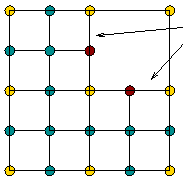
\includegraphics[height=.25\textheight]{graph/hanging}
    \end{center}
  \item storage of mesh hierarchy for multigrid
  \end{itemize}
\end{frame}

%%%%%%%%%%%%%%%%%%%%%%%%%%%%%%%%%%%%%%%%%%%%%%%%%%%%%%%%%%%%%%%%%%%%%% 
\subsection{Shape functions}
\begin{frame}
  \frametitle{Shape functions}
  \begin{itemize}
  \item $H^1$-conforming $Q_k$
  \item $H^{\text{div}}$-conforming RT$_k$, BDM$_k$
  \item $H^{\text{curl}}$-conforming Nedelec$_k$ (first family)
  \item discontinuous $Q_k$, $P_k$, vector elements
  \item support for implementation of further elements
  \end{itemize}
\end{frame}

%%%%%%%%%%%%%%%%%%%%%%%%%%%%%%%%%%%%%%%%%%%%%%%%%%%%%%%%%%%%%%%%%%%%%% 
\subsection{Degrees of freedom}
\begin{frame}
  \frametitle{Degrees of freedom}
  \begin{itemize}
  \item Element ``topology'' gets converted to ``global degrees
    of freedom''
  \item Generalized $hp$-methods
  \item Constraint operators for hanging nodes
  \item Level hierarchies of arbitrary elements
  \item Generic iterators to build matrices on cells and faces
  \end{itemize}
\end{frame}

%%%%%%%%%%%%%%%%%%%%%%%%%%%%%%%%%%%%%%%%%%%%%%%%%%%%%%%%%%%%%%%%%%%%%% 
\subsection{Systems of PDE}
\begin{frame}
  \frametitle{Systems of PDE}
  \begin{itemize}
  \item ``System elements'' simplify the implementation of systems of
    PDE
    \begin{itemize}
    \item Most data handling like for single equations
    \item Only local integrators have to change
    \end{itemize}
  \item Block vectors allow separation of equations
    \begin{itemize}
    \item Block preconditioners
    \item Projection schemes
    \end{itemize}
  \end{itemize}
\end{frame}

%%%%%%%%%%%%%%%%%%%%%%%%%%%%%%%%%%%%%%%%%%%%%%%%%%%%%%%%%%%%%%%%%%%%%% 
\subsection{Linear algebra}
\begin{frame}
  \frametitle{Linear algebra}
  \begin{itemize}
  \item Vectors and sparse matrices
  \item Elimination of hanging nodes
  \item Krylov space solvers: cg, GMRES, MinRes, Bicgstab, TFQMR
  \item Point and block relaxation
    \pause
  \item Multilevel support
  \item Block systems and Schur complements
    \pause
  \item Umfpack
  \item Interfaces to Trilinos, Lapack, Petsc, Slepc
    \pause
  \item Support for matrix free linear algebra work in progress
  \end{itemize}
\end{frame}

%%%%%%%%%%%%%%%%%%%%%%%%%%%%%%%%%%%%%%%%%%%%%%%%%%%%%%%%%%%%%%%%%%%%%% 
\subsection{Pre- and postprocessing}
\begin{frame}
  \frametitle{Pre- and postprocessing}
  \begin{itemize}
  \item<+-> Input drivers for several grid generators
    \begin{itemize}
    \item BAMG, MGF, GMSH, Salome, Cubit
    \item Graphic formats: UCD, Tecplot
    \end{itemize}
  \item<+-> Graphical output split into cell patches
    \begin{itemize}
    \item Drivers for VTK, UCD, OpenDX, gnuplot, Postscript, Tecplot, SVG
    \item Output for higher order elements
    \item New backends easily implemented
    \end{itemize}
  \end{itemize}
\end{frame}

%%%%%%%%%%%%%%%%%%%%%%%%%%%%%%%%%%%%%%%%%%%%%%%%%%%%%%%%%%%%%%%%%%%%%%
\begin{frame}
  \frametitle{The main classes}
  \centering
  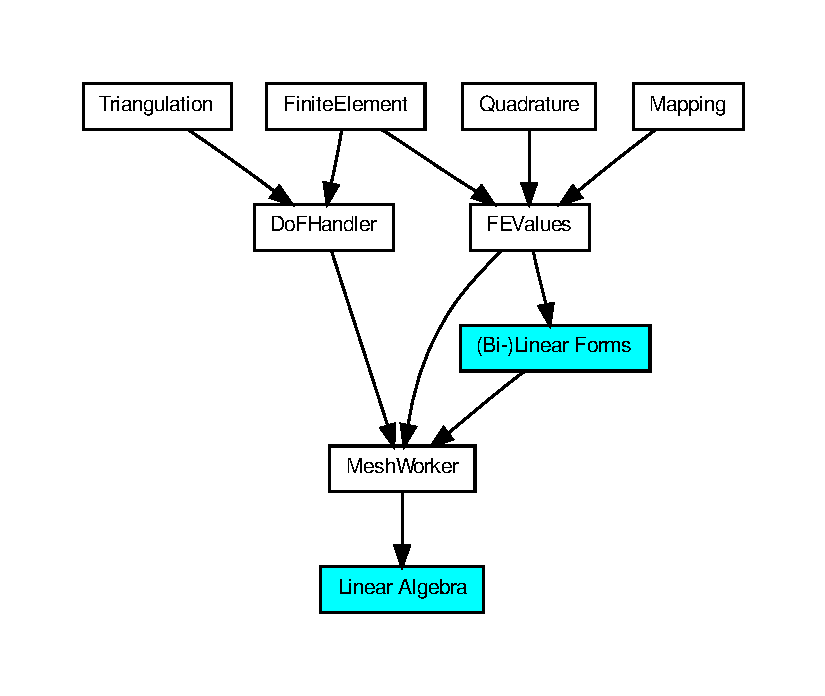
\includegraphics[height=.99\textheight]{graph/structure}
\end{frame}

%%%%%%%%%%%%%%%%%%%%%%%%%%%%%%%%%%%%%%%%%%%%%%%%%%%%%%%%%%%%%%%%%%%%%%
\begin{frame}
  \frametitle{The tutorial structure}

  \centering
  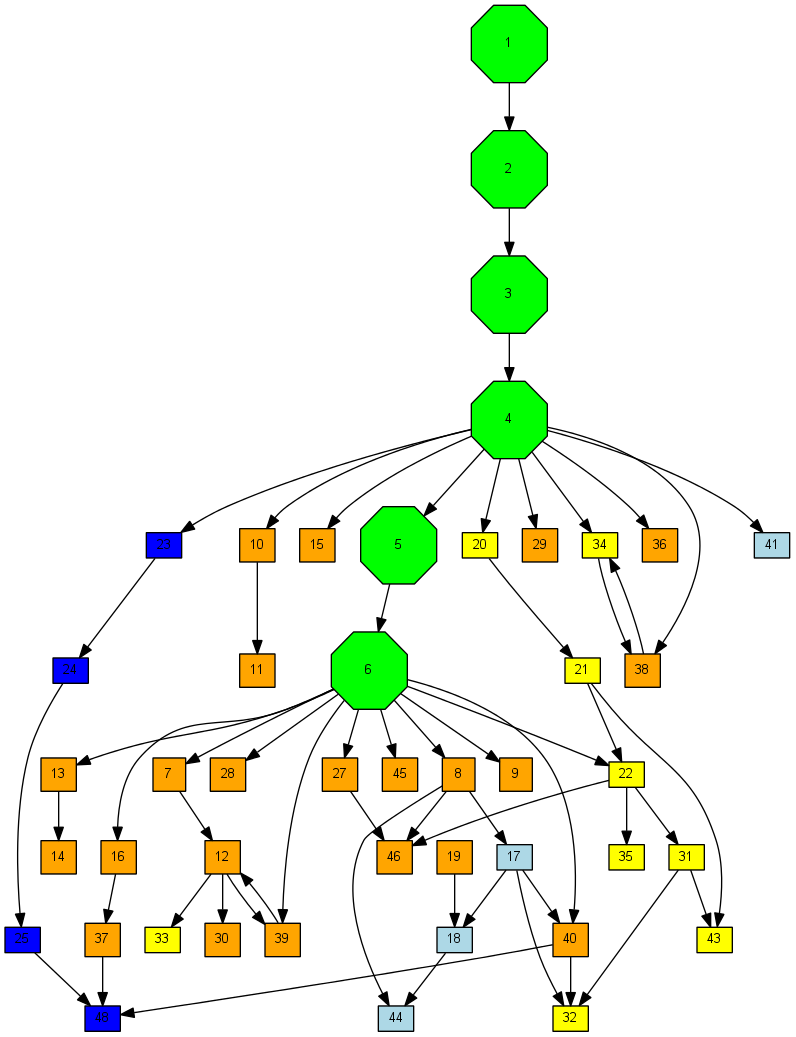
\includegraphics[height=.99\textheight]{graph/tutorial}

\end{frame}


%%% Local Variables: 
%%% mode: latex
%%% TeX-master: "slides"
%%% End: 
